\documentclass[hyperref,UTF8]{ctexart}
\usepackage{hyperref}

\usepackage{geometry}
\geometry{a4paper,scale=0.7}
\usepackage{tikz}
\usepackage{graphicx}
\usepackage{amsmath}
\usepackage{gnuplot-lua-tikz}
\usetikzlibrary{positioning, shapes.geometric}

\title{作业六: 一元二次方程在实数域上的求解}


\author{邵盛栋 \\ 信息与计算科学 3200103951}

\begin{document}
	\maketitle
	\textbf{一元二次方程式}是只含有一个未知数,并且未知数的最高次数是二次的多项式方程。
	
	一元二次方程式的一般形式是:
	\[ax^{2}+bx+c=0\qquad (a\neq 0)\]
	其中,$ ax^{2} $是二次项,$ bx $是一次项,$ c $是常数项。
	
	图\ref{fig:1}是求解一元二次方程求解的算法流程图:
	\begin{figure}[htpb]
		\centering
		\begin{tikzpicture}[node distance=20pt]
			\node[draw, rounded corners]                        (start)   {开始};
			\node[draw, below=of start]                         (step 1)  {输入三个数:a,b,c};
			\node[draw, diamond, below=of step 1]                        (step 2)  {$b^{2}-4ac>0$};
			\node[draw, below=of step 2]     (choice3)  {$ x=-\dfrac{b}{2a} $};
			\node[draw, left=30pt of choice3]     (choice1)  {$ x_{1}=-\dfrac{b-\sqrt{b^{2}-4ac>0}}{2a},x_{2}=-\dfrac{b+\sqrt{b^{2}-4ac>0}}{2a} $};
			\node[draw, right=30pt of choice3]     (choice2)  {$ x=-\dfrac{b}{2a} $};
			\node[draw, below=of choice3]                   (input2)  {输出x};
			\node[draw, left=30pt of input2]     (input1)  {输出x1,x2};
			\node[draw, below=of choice2]     (input3)  {无解};
			\node[draw, rounded corners, below=20pt of input2]  (end)     {结束};
			
			\draw[->] (start)  -- (step 1);
			\draw[->] (step 1) -- (step 2);
			\draw[->] (step 2) -- node[above] {Yes}  (step 2-|choice1) -> (choice1);
			\draw[->] (step 2) -- node[above] {No}  (step 2-|choice2) -> (choice2);
			\draw[->] (choice1) -- (choice1|-input1) -> (input1);
			\draw[->] (choice2) -- node[above] {Yes} (choice3);
			\draw[->] (choice2) -- node[right] {No} (input3);
			\draw[->] (choice3) -- (input2);
			\draw[->] (input1) -- (input1|-end) -> (end);
			\draw[->] (input2) -- (end);
			\draw[->] (input3) -- (input3|-end) -> (end);
		\end{tikzpicture}
		\caption{一元二次方程求解流程图}
		\label{fig:1}
	\end{figure}
	\newpage
	图\ref{fig:2}是一元二次方程解的三种情况的示意图:
	\begin{figure}[ht!]
		\centering
		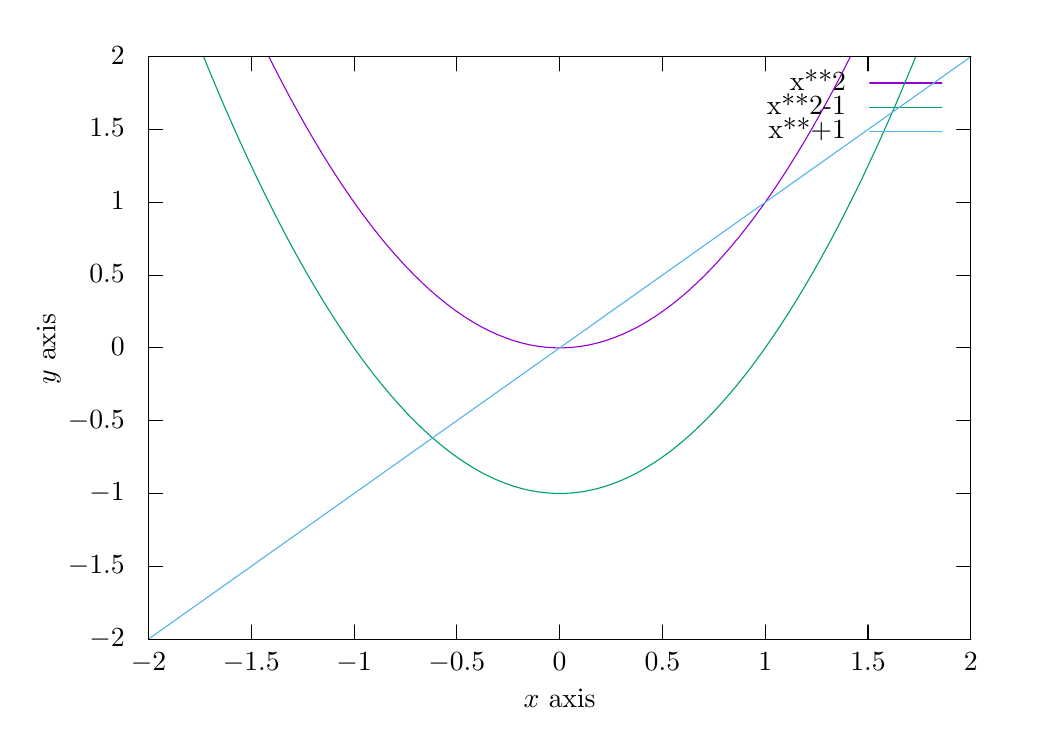
\begin{tikzpicture}[gnuplot]
			\path (0.000,0.000) rectangle (12.500,8.750);
			\gpcolor{color=gp lt color border}
			\gpsetlinetype{gp lt border}
			\gpsetdashtype{gp dt solid}
			\gpsetlinewidth{1.00}
			\draw[gp path] (1.504,0.985)--(1.684,0.985);
			\draw[gp path] (11.947,0.985)--(11.767,0.985);
			\node[gp node right] at (1.320,0.985) {$-2$};
			\draw[gp path] (1.504,1.910)--(1.684,1.910);
			\draw[gp path] (11.947,1.910)--(11.767,1.910);
			\node[gp node right] at (1.320,1.910) {$-1.5$};
			\draw[gp path] (1.504,2.834)--(1.684,2.834);
			\draw[gp path] (11.947,2.834)--(11.767,2.834);
			\node[gp node right] at (1.320,2.834) {$-1$};
			\draw[gp path] (1.504,3.759)--(1.684,3.759);
			\draw[gp path] (11.947,3.759)--(11.767,3.759);
			\node[gp node right] at (1.320,3.759) {$-0.5$};
			\draw[gp path] (1.504,4.683)--(1.684,4.683);
			\draw[gp path] (11.947,4.683)--(11.767,4.683);
			\node[gp node right] at (1.320,4.683) {$0$};
			\draw[gp path] (1.504,5.608)--(1.684,5.608);
			\draw[gp path] (11.947,5.608)--(11.767,5.608);
			\node[gp node right] at (1.320,5.608) {$0.5$};
			\draw[gp path] (1.504,6.532)--(1.684,6.532);
			\draw[gp path] (11.947,6.532)--(11.767,6.532);
			\node[gp node right] at (1.320,6.532) {$1$};
			\draw[gp path] (1.504,7.457)--(1.684,7.457);
			\draw[gp path] (11.947,7.457)--(11.767,7.457);
			\node[gp node right] at (1.320,7.457) {$1.5$};
			\draw[gp path] (1.504,8.381)--(1.684,8.381);
			\draw[gp path] (11.947,8.381)--(11.767,8.381);
			\node[gp node right] at (1.320,8.381) {$2$};
			\draw[gp path] (1.504,0.985)--(1.504,1.165);
			\draw[gp path] (1.504,8.381)--(1.504,8.201);
			\node[gp node center] at (1.504,0.677) {$-2$};
			\draw[gp path] (2.809,0.985)--(2.809,1.165);
			\draw[gp path] (2.809,8.381)--(2.809,8.201);
			\node[gp node center] at (2.809,0.677) {$-1.5$};
			\draw[gp path] (4.115,0.985)--(4.115,1.165);
			\draw[gp path] (4.115,8.381)--(4.115,8.201);
			\node[gp node center] at (4.115,0.677) {$-1$};
			\draw[gp path] (5.420,0.985)--(5.420,1.165);
			\draw[gp path] (5.420,8.381)--(5.420,8.201);
			\node[gp node center] at (5.420,0.677) {$-0.5$};
			\draw[gp path] (6.726,0.985)--(6.726,1.165);
			\draw[gp path] (6.726,8.381)--(6.726,8.201);
			\node[gp node center] at (6.726,0.677) {$0$};
			\draw[gp path] (8.031,0.985)--(8.031,1.165);
			\draw[gp path] (8.031,8.381)--(8.031,8.201);
			\node[gp node center] at (8.031,0.677) {$0.5$};
			\draw[gp path] (9.336,0.985)--(9.336,1.165);
			\draw[gp path] (9.336,8.381)--(9.336,8.201);
			\node[gp node center] at (9.336,0.677) {$1$};
			\draw[gp path] (10.642,0.985)--(10.642,1.165);
			\draw[gp path] (10.642,8.381)--(10.642,8.201);
			\node[gp node center] at (10.642,0.677) {$1.5$};
			\draw[gp path] (11.947,0.985)--(11.947,1.165);
			\draw[gp path] (11.947,8.381)--(11.947,8.201);
			\node[gp node center] at (11.947,0.677) {$2$};
			\draw[gp path] (1.504,8.381)--(1.504,0.985)--(11.947,0.985)--(11.947,8.381)--cycle;
			\node[gp node center,rotate=-270] at (0.246,4.683) {$y$ axis};
			\node[gp node center] at (6.725,0.215) {$x$ axis};
			\node[gp node right] at (10.479,8.047) {x**2};
			\gpcolor{rgb color={0.580,0.000,0.827}}
			\draw[gp path] (10.663,8.047)--(11.579,8.047);
			\draw[gp path] (3.034,8.381)--(3.086,8.276)--(3.192,8.070)--(3.297,7.871)--(3.403,7.678)%
			--(3.508,7.491)--(3.614,7.310)--(3.719,7.135)--(3.825,6.966)--(3.930,6.803)--(4.036,6.646)%
			--(4.141,6.495)--(4.247,6.350)--(4.352,6.211)--(4.458,6.078)--(4.563,5.952)--(4.669,5.831)%
			--(4.774,5.716)--(4.880,5.607)--(4.985,5.505)--(5.090,5.408)--(5.196,5.318)--(5.301,5.233)%
			--(5.407,5.155)--(5.512,5.082)--(5.618,5.016)--(5.723,4.955)--(5.829,4.901)--(5.934,4.853)%
			--(6.040,4.811)--(6.145,4.774)--(6.251,4.744)--(6.356,4.720)--(6.462,4.702)--(6.567,4.690)%
			--(6.673,4.684)--(6.778,4.684)--(6.884,4.690)--(6.989,4.702)--(7.095,4.720)--(7.200,4.744)%
			--(7.306,4.774)--(7.411,4.811)--(7.517,4.853)--(7.622,4.901)--(7.728,4.955)--(7.833,5.016)%
			--(7.939,5.082)--(8.044,5.155)--(8.150,5.233)--(8.255,5.318)--(8.361,5.408)--(8.466,5.505)%
			--(8.571,5.607)--(8.677,5.716)--(8.782,5.831)--(8.888,5.952)--(8.993,6.078)--(9.099,6.211)%
			--(9.204,6.350)--(9.310,6.495)--(9.415,6.646)--(9.521,6.803)--(9.626,6.966)--(9.732,7.135)%
			--(9.837,7.310)--(9.943,7.491)--(10.048,7.678)--(10.154,7.871)--(10.259,8.070)--(10.365,8.276)%
			--(10.417,8.381);
			\gpcolor{color=gp lt color border}
			\node[gp node right] at (10.479,7.739) {x**2-1};
			\gpcolor{rgb color={0.000,0.620,0.451}}
			\draw[gp path] (10.663,7.739)--(11.579,7.739);
			\draw[gp path] (2.204,8.381)--(2.242,8.286)--(2.348,8.033)--(2.453,7.785)--(2.559,7.544)%
			--(2.664,7.308)--(2.770,7.079)--(2.875,6.855)--(2.981,6.638)--(3.086,6.427)--(3.192,6.221)%
			--(3.297,6.022)--(3.403,5.829)--(3.508,5.642)--(3.614,5.461)--(3.719,5.286)--(3.825,5.117)%
			--(3.930,4.954)--(4.036,4.797)--(4.141,4.646)--(4.247,4.501)--(4.352,4.362)--(4.458,4.229)%
			--(4.563,4.103)--(4.669,3.982)--(4.774,3.867)--(4.880,3.758)--(4.985,3.656)--(5.090,3.559)%
			--(5.196,3.469)--(5.301,3.384)--(5.407,3.306)--(5.512,3.233)--(5.618,3.167)--(5.723,3.106)%
			--(5.829,3.052)--(5.934,3.004)--(6.040,2.962)--(6.145,2.925)--(6.251,2.895)--(6.356,2.871)%
			--(6.462,2.853)--(6.567,2.841)--(6.673,2.835)--(6.778,2.835)--(6.884,2.841)--(6.989,2.853)%
			--(7.095,2.871)--(7.200,2.895)--(7.306,2.925)--(7.411,2.962)--(7.517,3.004)--(7.622,3.052)%
			--(7.728,3.106)--(7.833,3.167)--(7.939,3.233)--(8.044,3.306)--(8.150,3.384)--(8.255,3.469)%
			--(8.361,3.559)--(8.466,3.656)--(8.571,3.758)--(8.677,3.867)--(8.782,3.982)--(8.888,4.103)%
			--(8.993,4.229)--(9.099,4.362)--(9.204,4.501)--(9.310,4.646)--(9.415,4.797)--(9.521,4.954)%
			--(9.626,5.117)--(9.732,5.286)--(9.837,5.461)--(9.943,5.642)--(10.048,5.829)--(10.154,6.022)%
			--(10.259,6.221)--(10.365,6.427)--(10.470,6.638)--(10.576,6.855)--(10.681,7.079)--(10.787,7.308)%
			--(10.892,7.544)--(10.998,7.785)--(11.103,8.033)--(11.209,8.286)--(11.247,8.381);
			\gpcolor{color=gp lt color border}
			\node[gp node right] at (10.479,7.431) {x**+1};
			\gpcolor{rgb color={0.337,0.706,0.914}}
			\draw[gp path] (10.663,7.431)--(11.579,7.431);
			\draw[gp path] (1.504,0.985)--(1.609,1.060)--(1.715,1.134)--(1.820,1.209)--(1.926,1.284)%
			--(2.031,1.359)--(2.137,1.433)--(2.242,1.508)--(2.348,1.583)--(2.453,1.657)--(2.559,1.732)%
			--(2.664,1.807)--(2.770,1.881)--(2.875,1.956)--(2.981,2.031)--(3.086,2.106)--(3.192,2.180)%
			--(3.297,2.255)--(3.403,2.330)--(3.508,2.404)--(3.614,2.479)--(3.719,2.554)--(3.825,2.629)%
			--(3.930,2.703)--(4.036,2.778)--(4.141,2.853)--(4.247,2.927)--(4.352,3.002)--(4.458,3.077)%
			--(4.563,3.152)--(4.669,3.226)--(4.774,3.301)--(4.880,3.376)--(4.985,3.450)--(5.090,3.525)%
			--(5.196,3.600)--(5.301,3.674)--(5.407,3.749)--(5.512,3.824)--(5.618,3.899)--(5.723,3.973)%
			--(5.829,4.048)--(5.934,4.123)--(6.040,4.197)--(6.145,4.272)--(6.251,4.347)--(6.356,4.422)%
			--(6.462,4.496)--(6.567,4.571)--(6.673,4.646)--(6.778,4.720)--(6.884,4.795)--(6.989,4.870)%
			--(7.095,4.944)--(7.200,5.019)--(7.306,5.094)--(7.411,5.169)--(7.517,5.243)--(7.622,5.318)%
			--(7.728,5.393)--(7.833,5.467)--(7.939,5.542)--(8.044,5.617)--(8.150,5.692)--(8.255,5.766)%
			--(8.361,5.841)--(8.466,5.916)--(8.571,5.990)--(8.677,6.065)--(8.782,6.140)--(8.888,6.214)%
			--(8.993,6.289)--(9.099,6.364)--(9.204,6.439)--(9.310,6.513)--(9.415,6.588)--(9.521,6.663)%
			--(9.626,6.737)--(9.732,6.812)--(9.837,6.887)--(9.943,6.962)--(10.048,7.036)--(10.154,7.111)%
			--(10.259,7.186)--(10.365,7.260)--(10.470,7.335)--(10.576,7.410)--(10.681,7.485)--(10.787,7.559)%
			--(10.892,7.634)--(10.998,7.709)--(11.103,7.783)--(11.209,7.858)--(11.314,7.933)--(11.420,8.007)%
			--(11.525,8.082)--(11.631,8.157)--(11.736,8.232)--(11.842,8.306)--(11.947,8.381);
			\gpcolor{color=gp lt color border}
			\draw[gp path] (1.504,8.381)--(1.504,0.985)--(11.947,0.985)--(11.947,8.381)--cycle;
			%% coordinates of the plot area
			\gpdefrectangularnode{gp plot 1}{\pgfpoint{1.504cm}{0.985cm}}{\pgfpoint{11.947cm}{8.381cm}}
		\end{tikzpicture}
		\caption{一元二次方程解的三种情况示意图}
		\label{fig:2}
	\end{figure}
\end{document}
